%=============================================================================
\section{Databáze}
%=============================================================================

\subsection*{Obecné pojmy}

\textbf{Databáze} je organizovaný systém souborů pro ukládání dat. Tyto soubory jsou mezi sebou navzájem
propojeny. V širším smyslu jsou součástí databáze i softwarové prostředky, které umožňují manipulaci
s uloženými daty a přístup k nim. Tento software se v české odborné literatuře nazývá \textbf{systém řízení
báze dat (SŘBD)}. Běžně se označením databáze myslí jak uložená data, tak i software.

\begin{itemize}
  \item \textbf{data} -- formalizované a fyzicky zaznamenané znalosti, poznatky, zkušenosti, výsledky pozorování
  \item \textbf{informace} -- smysluplná interpretace dat
  \item \textbf{databáze} -- integrovaná počítačově zpracovaná množina persistentních dat
  \item \textbf{relační model dat} -- data jsou uložena v tabulkách (relacích); každý řádek je jedna
    entita, každý sloupec je atribut. Matematický základ tvoří predikátová logika prvního řádu.
    Existují dva ekvivalentní způsoby jak se na manipulaci s daty dívat:
    \begin{itemize}
      \item \textbf{Relační algebra} -- \textit{procedurální} přístup; popisuje \textit{jak} data získat pomocí
        operátorů: $\sigma$ (selekce řádků), $\pi$ (projekce sloupců), $\bowtie$ (spojení tabulek),
        $\cup$ (sjednocení), $-$ (rozdíl). Příklad: ``z tabulky zaměstnanců vyber sloupce jméno a plat,
        kde plat > 50\,000'' = $\pi_{\text{jméno, plat}}(\sigma_{\text{plat}>50000}(\text{zamestnanci}))$
      \item \textbf{Relační kalkul} -- \textit{deklarativní} přístup; popisuje \textit{co} chceme
        (ne jak to získat). SQL je v podstatě syntaktický cukr nad relačním kalkulem -- napíšete
        \texttt{SELECT jmeno, plat FROM zamestnanci WHERE plat > 50000} a databázový stroj sám
        rozhodne, jak dotaz vykoná
    \end{itemize}
    Oba přístupy jsou ekvivalentní (Coddův teorém) -- vše co jde vyjádřit algebrou, jde vyjádřit
    i kalkulem a naopak
  \item \textbf{dotazovací jazyk} -- slouží pro získání dat z databáze; v relační databázi je odpovědí relace,
    jejíž n-tice splňují nadefinované podmínky
  \item \textbf{systém řízení bází dat (SŘBD / DBMS)} -- množina programových prostředků, která umožňuje:
    vytvoření databáze, použití databáze (manipulace s daty), údržbu a správu databáze
  \item \textbf{databázový systém (DBS)} -- SŘBD + databáze
\end{itemize}

\subsubsection*{Dělení databází podle typu}

\begin{enumerate}
  \item \textbf{Relační databáze} -- nejčastěji používaný typ; data modelována pomocí tabulek s fixní strukturou
    propojených pomocí relací. Příklady: Oracle, MySQL, PostgreSQL, MS SQL Server.

  \item \textbf{NoSQL databáze} -- bez tabulek, nestrukturované; rychlejší a škálovatelnější.
    Ukládání dat do JSON/BSON. Příklady: MongoDB, CouchDB, Amazon DynamoDB.

  \item \textbf{Specializované databáze}:
    \begin{itemize}
      \item \textit{Graph Databases} -- neo4j; grafové struktury pro modelování sítí
      \item \textit{Key-Value} -- Redis, Memcached; jedna hodnota pro daný klíč (cache)
      \item \textit{Time-series} -- optimalizované pro časové řady dat
      \item \textit{Sloupcové} -- Cassandra, HBase; data ukládána po sloupcích
    \end{itemize}
\end{enumerate}

%=============================================================================
\subsection{Analýza, návrh a realizace databáze}
%=============================================================================

\subsubsection{Databázový systém a jeho vlastnosti}

\textbf{Databázový systém (DBS) = SŘBD + Databáze}

Důvody pro vznik databázových systémů:
\begin{itemize}
  \item \textbf{Vyšší datová abstrakce} -- SŘDB zahrnují manipulační jazyky pro práci s datovými strukturami vyšší úrovně
  \item \textbf{Nezávislost aplikačních programů} na změnách ve fyzickém uložení dat
  \item \textbf{Ochrana dat} před neoprávněným přístupem a poruchami
  \item \textbf{Odstranění redundance} -- každý údaj uložen pouze jedenkrát
  \item \textbf{Sdílení dat} -- data mohou být používána několika uživateli
  \item \textbf{Podpora transakčního zpracování}
  \item \textbf{Údržba integrity databáze}
\end{itemize}

\subsubsection{Metodologie analýzy a návrhu databáze -- P3A}

Návrh databáze vychází z principu tří architektur (\textbf{P3A}). Smyslem P3A je postupně upřesňovat
datový model tak, aby zcela odpovídal požadavkům využívané databázové technologie.

\textit{Příklad prolínající se všemi třemi úrovněmi: systém e-shopu (zákazníci, objednávky, produkty).}

\paragraph{1. Konceptuální model (model reality)}
Model obsahu datové základny na konceptuální úrovni -- nezávislý na technologii, bez datových typů.
\begin{itemize}
  \item \textbf{KSR} (Konceptuální schéma reality) -- hrubý model; základní entity, vztahy a atributy
  \item \textbf{KSD} (Konceptuální schéma dat) -- přesná specifikace; ER diagram (Entity-Relationship)
\end{itemize}

\begin{figure}[H]
\centering
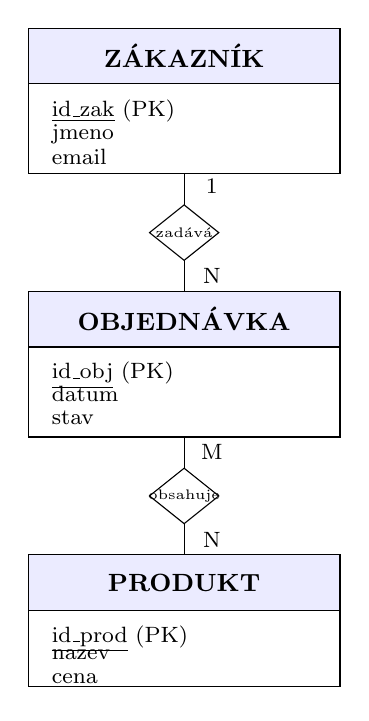
\begin{tikzpicture}[font=\small, scale=0.88]
  % ZAKAZNIK
  \draw[fill=blue!8] (0,5.6) rectangle (4.5,6.4);
  \node[font=\small\bfseries] at (2.25,6.0) {ZÁKAZNÍK};
  \draw (0,4.3) rectangle (4.5,5.6);
  \node[anchor=north west,font=\footnotesize] at (0.2,5.5) {\underline{id\_zak} (PK)};
  \node[anchor=north west,font=\footnotesize] at (0.2,5.15) {jmeno};
  \node[anchor=north west,font=\footnotesize] at (0.2,4.8) {email};
  % line + cardinality
  \draw (2.25,4.3) -- (2.25,3.85);
  \node[font=\footnotesize] at (2.65,4.12) {1};
  % relationship diamond "zadava"
  \draw (1.75,3.45) -- (2.25,3.85) -- (2.75,3.45) -- (2.25,3.05) -- cycle;
  \node[font=\tiny] at (2.25,3.45) {zadává};
  % line + cardinality
  \draw (2.25,3.05) -- (2.25,2.6);
  \node[font=\footnotesize] at (2.65,2.83) {N};
  % OBJEDNAVKA
  \draw[fill=blue!8] (0,1.8) rectangle (4.5,2.6);
  \node[font=\small\bfseries] at (2.25,2.2) {OBJEDNÁVKA};
  \draw (0,0.5) rectangle (4.5,1.8);
  \node[anchor=north west,font=\footnotesize] at (0.2,1.72) {\underline{id\_obj} (PK)};
  \node[anchor=north west,font=\footnotesize] at (0.2,1.37) {datum};
  \node[anchor=north west,font=\footnotesize] at (0.2,1.02) {stav};
  % line + cardinality
  \draw (2.25,0.5) -- (2.25,0.05);
  \node[font=\footnotesize] at (2.65,0.28) {M};
  % relationship diamond "obsahuje"
  \draw (1.75,-0.35) -- (2.25,0.05) -- (2.75,-0.35) -- (2.25,-0.75) -- cycle;
  \node[font=\tiny] at (2.25,-0.35) {obsahuje};
  % line + cardinality
  \draw (2.25,-0.75) -- (2.25,-1.2);
  \node[font=\footnotesize] at (2.65,-0.98) {N};
  % PRODUKT
  \draw[fill=blue!8] (0,-2.0) rectangle (4.5,-1.2);
  \node[font=\small\bfseries] at (2.25,-1.6) {PRODUKT};
  \draw (0,-3.1) rectangle (4.5,-2.0);
  \node[anchor=north west,font=\footnotesize] at (0.2,-2.08) {\underline{id\_prod} (PK)};
  \node[anchor=north west,font=\footnotesize] at (0.2,-2.43) {nazev};
  \node[anchor=north west,font=\footnotesize] at (0.2,-2.78) {cena};
\end{tikzpicture}
\caption{Konceptuální model -- ER diagram e-shopu}
\label{fig:erd}
\end{figure}

\paragraph{2. Logický (technologický) model}
Konceptuální schéma se transformuje do relačních tabulek. Vztah M:N (OBJEDNÁVKA--PRODUKT)
se rozloží na vazební tabulku POLOŽKA se dvěma cizími klíči.

\begin{itemize}
  \item Každá entitní množina $\to$ relační tabulka; identifikátory $\to$ primární klíč
  \item Vztah 1:N $\to$ cizí klíč (FK) na straně N
  \item Vztah M:N $\to$ vazební tabulka se dvěma cizími klíči
  \item Generalizace/specializace $\to$ varianty: jedna tabulka pro celou hierarchii, nebo tabulky na úrovni specializací
\end{itemize}

\textbf{Výsledné schéma} (PK podtrženo, FK šipkou):

\begin{center}
\begin{tabular}{ll}
\toprule
\textbf{Tabulka} & \textbf{Atributy} \\
\midrule
ZÁKAZNÍK & \underline{id\_zak}, jmeno, email \\
OBJEDNÁVKA & \underline{id\_obj}, id\_zak $\to$ ZÁKAZNÍK, datum, stav \\
PRODUKT & \underline{id\_prod}, nazev, cena \\
POLOŽKA & \underline{id\_obj} $\to$ OBJEDNÁVKA, \underline{id\_prod} $\to$ PRODUKT, mnozstvi \\
\bottomrule
\end{tabular}
\end{center}

Cíle logického modelu: věrný obraz reality, interní konzistence, minimalizace redundance, maximalizace stability.
Sada normálních forem: 1NF, 2NF, 3NF, BCNF, 4NF, 5NF.

\paragraph{3. Fyzický (implementační) model}
Logický model se přepíše do konkrétního DDL jazyka cílové databáze -- přidají se datové typy,
omezení, indexy a optimalizace pro výkon.

\begin{itemize}
  \item \textbf{Způsob uložení dat:} sekvenční (pro zálohy), přímé (hashing -- adresa záznamu = f(PK))
  \item \textbf{Způsob přístupu k datům:} sekvenční, přímé, indexy
\end{itemize}

\begin{lstlisting}[language=SQL, caption=Fyzický model -- CREATE TABLE (PostgreSQL)]
CREATE TABLE zakaznik (
    id_zak  INT          PRIMARY KEY,
    jmeno   VARCHAR(100) NOT NULL,
    email   VARCHAR(200) UNIQUE NOT NULL
);

CREATE TABLE objednavka (
    id_obj  INT  PRIMARY KEY,
    id_zak  INT  NOT NULL REFERENCES zakaznik(id_zak),
    datum   DATE NOT NULL DEFAULT CURRENT_DATE,
    stav    VARCHAR(20) NOT NULL DEFAULT 'nova'
);
-- Index pro rychlé hledání vsech objednavek zakaznika
CREATE INDEX idx_obj_zak ON objednavka(id_zak);

CREATE TABLE produkt (
    id_prod  INT            PRIMARY KEY,
    nazev    VARCHAR(200)   NOT NULL,
    cena     DECIMAL(10,2)  NOT NULL CHECK (cena > 0)
);

-- Vazebni tabulka pro vztah M:N (objednavka <-> produkt)
CREATE TABLE polozka (
    id_obj   INT REFERENCES objednavka(id_obj) ON DELETE CASCADE,
    id_prod  INT REFERENCES produkt(id_prod),
    mnozstvi INT NOT NULL DEFAULT 1 CHECK (mnozstvi > 0),
    PRIMARY KEY (id_obj, id_prod)   -- slozeny PK
);
\end{lstlisting}

\subsubsection{Normalizace databáze}

\textbf{Normalizace} je proces postupného odstraňování redundancí a anomálií z databázového schématu.
Každá normální forma buduje na předchozí -- pokud je tabulka v 3NF, je automaticky i v 2NF a 1NF.

\textbf{Proč normalizovat?} Bez normalizace vznikají \textit{anomálie}:
\begin{itemize}
  \item \textbf{Vkládací anomálie} -- nelze vložit data bez jiných dat (nelze přidat oddělení bez zaměstnance)
  \item \textbf{Aktualizační anomálie} -- změna jednoho faktu vyžaduje UPDATE na více řádcích najednou
  \item \textbf{Mazací anomálie} -- smazání řádku odstraní nezávislou informaci
\end{itemize}

%--- 1NF ---
\paragraph{1. normální forma (1NF)}
\textbf{Pravidlo:} Každá buňka tabulky obsahuje právě jednu \textit{atomickou} (nedělitelnou) hodnotu.
Neexistují opakující se skupiny atributů ani seznamy hodnot v jedné buňce.

\smallskip
\textit{Porušení -- seznam hodnot v buňce:}
\begin{center}\footnotesize
\begin{tabular}{lll}
\toprule
id\_zam & jmeno & telefony \\
\midrule
1 & Jan Novák & \textbf{777\,111\,222, 777\,333\,444} \\
2 & Eva Černá & \textbf{603\,555\,666} \\
\bottomrule
\end{tabular}
\end{center}

\textit{Oprava -- přesun vícehodnotového atributu do vlastní tabulky:}
\begin{center}\footnotesize
\begin{tabular}{ll}
\toprule
\multicolumn{2}{c}{\textbf{ZAMESTNANEC}} \\
\midrule
\underline{id\_zam} & jmeno \\
1 & Jan Novák \\
2 & Eva Černá \\
\bottomrule
\end{tabular}
\quad
\begin{tabular}{ll}
\toprule
\multicolumn{2}{c}{\textbf{ZAM\_TELEFON}} \\
\midrule
\underline{id\_zam} & \underline{telefon} \\
1 & 777\,111\,222 \\
1 & 777\,333\,444 \\
2 & 603\,555\,666 \\
\bottomrule
\end{tabular}
\end{center}

%--- 2NF ---
\paragraph{2. normální forma (2NF)}
\textbf{Pravidlo:} Je v 1NF a každý neklíčový atribut závisí na \textit{celém} složeném PK, ne jen na jeho části.
(Relevantní pouze pro tabulky se složeným primárním klíčem.)

\smallskip
\textit{Porušení -- částečná závislost (nazev\_prod závisí jen na id\_prod, ne na celém PK):}
\begin{center}\footnotesize
\begin{tabular}{lllll}
\toprule
\multicolumn{5}{c}{\textbf{POLOZKA} \quad PK = (\underline{id\_obj}, \underline{id\_prod})} \\
\midrule
id\_obj & id\_prod & mnozstvi & \textbf{nazev\_prod} & \textbf{cena} \\
\midrule
1 & 101 & 2 & Kniha Java & 599 \\
1 & 102 & 1 & Myš & 299 \\
2 & 101 & 1 & Kniha Java & 599 \\
\bottomrule
\end{tabular}
\end{center}
Problém: ``Kniha Java'' se opakuje -- změna názvu vyžaduje UPDATE na více řádcích.

\textit{Oprava -- oddělit atributy závislé jen na id\_prod:}
\begin{center}\footnotesize
\begin{tabular}{lll}
\toprule
\multicolumn{3}{c}{\textbf{POLOZKA}} \\
\midrule
\underline{id\_obj} & \underline{id\_prod} & mnozstvi \\
1 & 101 & 2 \\
1 & 102 & 1 \\
\bottomrule
\end{tabular}
\quad
\begin{tabular}{lll}
\toprule
\multicolumn{3}{c}{\textbf{PRODUKT}} \\
\midrule
\underline{id\_prod} & nazev\_prod & cena \\
101 & Kniha Java & 599 \\
102 & Myš & 299 \\
\bottomrule
\end{tabular}
\end{center}

%--- 3NF ---
\paragraph{3. normální forma (3NF)}
\textbf{Pravidlo:} Je v 2NF a neexistuje \textit{tranzitivní závislost} neklíčového atributu na PK.

\medskip
\begin{tcolorbox}[colback=yellow!15, colframe=orange!60, title=Co je tranzitivní závislost?]
Tranzitivní závislost nastane, když neklíčový atribut závisí na \textbf{jiném neklíčovém atributu}
místo přímo na PK. Jinými slovy: existuje řetěz $A \to B \to C$, kde $B$ není klíč.

\smallskip
Příklad: $\text{id\_zam} \to \text{id\_oddel} \to \text{nazev\_oddel}$

\textit{nazev\_oddel} neurčuje přímo PK (\textit{id\_zam}), ale prostřednictvím \textit{id\_oddel}.
\end{tcolorbox}

\smallskip
\textit{Porušení -- tranzitivní závislost přes id\_oddel:}
\begin{center}\footnotesize
\begin{tabular}{lllll}
\toprule
\multicolumn{5}{c}{\textbf{ZAMESTNANEC} \quad PK = \underline{id\_zam}} \\
\midrule
id\_zam & jmeno & id\_oddel & \textbf{nazev\_oddel} & \textbf{budova} \\
\midrule
1 & Jan Novák & 10 & IT & A \\
2 & Eva Černá & 10 & IT & A \\
3 & Petr Bílý & 20 & Finance & B \\
\bottomrule
\end{tabular}
\end{center}

Závislosti: $\text{id\_zam} \to \text{id\_oddel}$ (přímá, OK) \quad
$\text{id\_oddel} \to \text{nazev\_oddel, budova}$ (id\_oddel \textbf{není klíč}!)

Problém: IT přestěhuje z budovy A do C $\Rightarrow$ musím aktualizovat \textbf{oba} řádky (Jan i Eva).
Pokud zapomenu jeden $\Rightarrow$ nekonzistence.

\textit{Oprava -- vytáhnout atributy závislé na id\_oddel do vlastní tabulky:}
\begin{center}\footnotesize
\begin{tabular}{lll}
\toprule
\multicolumn{3}{c}{\textbf{ZAMESTNANEC}} \\
\midrule
\underline{id\_zam} & jmeno & id\_oddel (FK) \\
1 & Jan Novák & 10 \\
2 & Eva Černá & 10 \\
\bottomrule
\end{tabular}
\quad
\begin{tabular}{lll}
\toprule
\multicolumn{3}{c}{\textbf{ODDELENI}} \\
\midrule
\underline{id\_oddel} & nazev\_oddel & budova \\
10 & IT & A \\
20 & Finance & B \\
\bottomrule
\end{tabular}
\end{center}
Přestěhování IT: jediný UPDATE v ODDELENI, žádná redundance.

%--- BCNF ---
\paragraph{Boyce-Coddova normální forma (BCNF)}
\textbf{Pravidlo:} Je v 3NF a pro každou netriviální funkční závislost $X \to Y$ musí být $X$
nadmnožinou \textit{kandidátního klíče} (superklíč). BCNF je přísnější než 3NF.

\smallskip
\textit{Porušení -- klasický příklad: rozvrh výuky.}
\begin{center}\footnotesize
\begin{tabular}{lll}
\toprule
\multicolumn{3}{c}{\textbf{ZKOUSENI}} \\
\midrule
\underline{student} & \underline{predmet} & ucitel \\
\midrule
Novák & Databáze & Dr.~Svátek \\
Černá & Databáze & Dr.~Svátek \\
Novák & Java & Ing.~Vojíř \\
\bottomrule
\end{tabular}
\end{center}

Funkční závislosti: $(student, predmet) \to ucitel$ (každý student má jednoho učitele per předmět)
a zároveň $ucitel \to predmet$ (každý učitel učí jen jeden předmět).
Kandidátní klíče: $\{student, predmet\}$ nebo $\{student, ucitel\}$.
Porušení: $ucitel \to predmet$, ale \textit{ucitel} samotný \textbf{není superklíč}.

\textit{Oprava:}
\begin{center}\footnotesize
\begin{tabular}{ll}
\toprule\textbf{UCITEL\_PREDMET}\\\midrule
\underline{ucitel} & predmet \\\midrule
Dr.~Svátek & Databáze \\
Ing.~Vojíř & Java \\
\bottomrule
\end{tabular}
\quad
\begin{tabular}{ll}
\toprule\textbf{STUDENT\_UCITEL}\\\midrule
\underline{student} & \underline{ucitel}\\\midrule
Novák & Dr.~Svátek \\
Černá & Dr.~Svátek \\
Novák & Ing.~Vojíř \\
\bottomrule
\end{tabular}
\end{center}

%--- 4NF ---
\paragraph{4. normální forma (4NF)}
\textbf{Pravidlo:} Je v BCNF a neobsahuje netriviální \textit{vícehodnotové závislosti} (MVD).

Vícehodnotová závislost $A \twoheadrightarrow B$ nastane, když jeden atribut $A$ určuje \textbf{nezávislou sadu}
hodnot $B$ bez ohledu na ostatní atributy.

\smallskip
\textit{Porušení -- dovednosti a certifikáty zaměstnance jsou na sobě nezávislé:}
\begin{center}\footnotesize
\begin{tabular}{lll}
\toprule
\multicolumn{3}{c}{\textbf{ZAM\_DOV\_CERT}} \\
\midrule
id\_zam & dovednost & certifikat \\
\midrule
1 & Java & ITSM \\
1 & Java & PMP \\
1 & SQL  & ITSM \\
1 & SQL  & PMP \\
\bottomrule
\end{tabular}
\end{center}

Jan (id\_zam=1) zná Java a SQL, a má certifikáty ITSM a PMP. Tyto fakty jsou \textbf{nezávislé} --
přidání nové dovednosti (Python) vyžaduje vložit 2 nové řádky (Python+ITSM, Python+PMP).

\textit{Oprava -- rozdělit na dvě tabulky:}
\begin{center}\footnotesize
\begin{tabular}{ll}
\toprule
\multicolumn{2}{c}{\textbf{ZAM\_DOVEDNOST}} \\
\midrule
\underline{id\_zam} & \underline{dovednost} \\
1 & Java \\ 1 & SQL \\
\bottomrule
\end{tabular}
\quad
\begin{tabular}{ll}
\toprule
\multicolumn{2}{c}{\textbf{ZAM\_CERTIFIKAT}} \\
\midrule
\underline{id\_zam} & \underline{certifikat} \\
1 & ITSM \\ 1 & PMP \\
\bottomrule
\end{tabular}
\end{center}

%--- 5NF ---
\paragraph{5. normální forma (5NF -- PJNF)}
\textbf{Pravidlo:} Je v 4NF a neobsahuje závislosti spojení (\textit{join dependency}) které nelze odvodit
z kandidátních klíčů. Tabulka je v 5NF tehdy, když ji \textbf{nelze bezztrátově rozložit} na menší tabulky.

5NF se uplatňuje u tříciferných (a vícenásobných) vztahů, kde ternární vazbu \textbf{nelze}
nahradit binárními vztahy bez ztráty informace.

\smallskip
\textit{Příklad: dodavatel -- produkt -- zákazník}
\begin{center}\footnotesize
\begin{tabular}{lll}
\toprule
dodavatel & produkt & zakaznik \\
\midrule
ACME & Tužka & Škola \\
ACME & Pero & Škola \\
Beta & Tužka & Firma \\
\bottomrule
\end{tabular}
\end{center}

Pokud platí obchodní pravidlo: \textit{``jestliže dodavatel D dodává produkt P, zákazník Z odebírá produkt P
a D prodává zákazníkovi Z, pak tuple (D,P,Z) musí existovat''}, pak lze tabulku bezztrátově rozložit
do tří binárních projekcí (DODAVATEL\_PRODUKT, PRODUKT\_ZAKAZNIK, DODAVATEL\_ZAKAZNIK) -- to je 5NF.

Pokud toto obchodní pravidlo neplatí, ternární tabulka je v 5NF a \textbf{nesmí se rozkládat}
(rozklad by způsobil spurious tuples při přirozeném joinu).

\smallskip
\textit{Poznámka: 4NF a 5NF se v praxi řeší vzácně -- většina reálných projektů cíluje na 3NF nebo BCNF.}

%--- Denormalizace ---
\paragraph{Denormalizace}
Záměrné porušování normalizace za účelem zvýšení výkonnosti systému:
\begin{itemize}
  \item \textbf{Výhody:} snižování potřeby joinů, uchování aktuálních hodnot odvozených atributů
  \item \textbf{Nevýhody:} pomalejší UPDATE/INSERT/DELETE, složitější zajištění integrity
\end{itemize}

\subsubsection{Integrita a transakce}

\paragraph{Integritní omezení}
\begin{itemize}
  \item \textbf{Entitní integrita} -- PK musí být UNIQUE a NOT NULL
  \item \textbf{Referenční integrita} -- FK odkazuje pouze na existující hodnoty PK
  \item \textbf{Doménová integrita} -- atribut obsahuje pouze přípustné hodnoty (CHECK, TRIGGER)
\end{itemize}

\paragraph{Transakce a vlastnosti ACID}
\begin{itemize}
  \item \textbf{A (Atomicity)} -- transakce proběhne celá nebo žádná část
  \item \textbf{C (Consistency)} -- DB přechází z jednoho konzistentního stavu do jiného
  \item \textbf{I (Isolation)} -- souběžné transakce jsou navzájem nezávislé
  \item \textbf{D (Durability)} -- efekty potvrzené transakce jsou trvale uloženy
\end{itemize}

\paragraph{BASE (NoSQL alternativa k ACID)}
NoSQL systémy upřednostňují dostupnost nad konzistencí (CAP teorém):
\begin{itemize}
  \item \textbf{BA (Basically Available)} -- systém vždy odpovídá, i kdyby data nebyla aktuální
  \item \textbf{S (Soft-state)} -- stav systému se může měnit i bez vstupu (postupná synchronizace)
  \item \textbf{E (Eventual consistency)} -- po dostatečné době bez nových zápisů se systém stane konzistentním
\end{itemize}

\paragraph{Izolace transakcí a problémy při souběžném přístupu}
Úrovně izolace (SQL standard) a problémy, které řeší:
\begin{itemize}
  \item \textbf{Dirty read} -- čtení nepotvrzených dat jiné transakce
  \item \textbf{Non-repeatable read} -- opakované čtení vrátí různé hodnoty (jiná transakce mezitím změnila)
  \item \textbf{Phantom read} -- dotaz vrátí jiné řádky při opakování (jiná transakce vložila/smazala)
  \item \textbf{Izolační úrovně:} READ UNCOMMITTED $<$ READ COMMITTED $<$ REPEATABLE READ $<$ SERIALIZABLE
\end{itemize}

\paragraph{Uváznutí (Deadlock)}
Situace, kdy dvě nebo více transakcí čekají na uvolnění zámků navzájem:
\begin{itemize}
  \item \textbf{Prevence} -- stanovení pořadí zamykání zdrojů
  \item \textbf{Detekce a obnova} -- DBMS detekuje cyklus v grafu čekání a jednu transakci přeruší (victim)
  \item \textbf{Timeout} -- transakce čekající příliš dlouho se automaticky ukončí
\end{itemize}

\paragraph{Obnova po selhání (Recovery)}
\begin{itemize}
  \item \textbf{Žurnál (Log)} -- záznamy o všech změnách (before-image, after-image)
  \item \textbf{UNDO} -- odvolání nepotvrzených transakcí (po pádu systému)
  \item \textbf{REDO} -- opakování potvrzených transakcí (obnovení po pádu)
  \item \textbf{Checkpoint} -- periodický zápis stavu paměti na disk; zkrátí dobu obnovy
\end{itemize}

\begin{itemize}
  \item \textbf{OLAP} (Online Analytical Processing) -- vícedimenzionální dotazy, datové sklady, historická data
  \item \textbf{OLTP} (Online Transaction Processing) -- velké množství malých transakcí (INSERT, UPDATE, DELETE)
\end{itemize}

\subsubsection{Indexy}

\textbf{Indexy} slouží ke zrychlení vyhledávání. Každý index zabírá místo v paměti a zpomaluje
operace INSERT/UPDATE nad indexovanými sloupci.

\begin{profesorbox}[Otázky profesorů k tématu: Analýza, návrh a realizace databáze]
\textbf{Komise: Svátek, Chlapek, Zbořil}
\begin{itemize}
  \item Jaký by měl být správný postup analýzy, návrhu a realizace databáze?
\end{itemize}
\textbf{Máša Petr, RNDr. Ing., Ph.D.}
\begin{itemize}
  \item Jaké budou problémy aplikace vysoce náročné na data, jak řešit databázi?
  \item Co se rozumí principem 3NF?
\end{itemize}
\textbf{Sládek Pavel, Ing., Ph.D.}
\begin{itemize}
  \item Jaké jsou druhy databází a jak fungují?
\end{itemize}
\textbf{Chudán David, Ing., Ph.D.}
\begin{itemize}
  \item Jak se typicky strukturovaná data ukládají? Jaké znáte typy databází?
  \item Jaké jsou rozdíly mezi formáty CSV, JSON a XML?
\end{itemize}
\textbf{Zeman Václav, Ing., Ph.D.}
\begin{itemize}
  \item Jak databáze zajistí konzistenci a integritu řešení?
\end{itemize}
\textbf{Strossa Petr, doc. RNDr., CSc.}
\begin{itemize}
  \item V čem se liší NoSQL od relačních databází?
  \item K čemu slouží indexy v databázi?
\end{itemize}
\textbf{Sudzina František, Mgr.\ et Mgr.\ Ing., Ph.D.}
\begin{itemize}
  \item Jaké jsou výhody databází v porovnání s tabulkami v Excelu?
\end{itemize}
\textbf{Maryška Miloš, doc. Ing., Ph.D.}
\begin{itemize}
  \item Co je normalizace a denormalizace dat?
\end{itemize}
\end{profesorbox}

%=============================================================================
\subsection{Datové modelování}
%=============================================================================

\textbf{Datové modelování} je proces vytváření abstraktního modelu toho, \textit{jaká data systém
potřebuje ukládat, jak jsou mezi sebou provázána a jaká omezení na ně platí.}
Provádí se \textbf{před} samotnou implementací databáze, podobně jako architekt kreslí plán budovy
před zahájením stavby.

\paragraph{Proč datové modelování potřebujeme?}
Bez datového modelu si vývojáři navrhnou tabulky intuitivně -- výsledkem bývají redundance,
chybějící vazby, problémy s integrací a nutnost drahých refaktoringů. Datový model:
\begin{itemize}
  \item přesně popisuje co systém o světě \textit{ví} (které entity evidujeme, jaké mají vlastnosti)
  \item zachytí \textbf{pravidla byznysu} jako omezení v databázi (zaměstnanec musí patřit do oddělení)
  \item slouží jako \textbf{společný jazyk} mezi analytiky, vývojáři a zákazníkem
  \item je vstupem pro normalizaci a fyzický návrh
\end{itemize}

\paragraph{Co datový model zachycuje?}
\begin{itemize}
  \item \textbf{Entity} -- věci, o kterých chceme ukládat data (zákazník, produkt, objednávka)
  \item \textbf{Atributy} -- vlastnosti entit (jméno zákazníka, cena produktu)
  \item \textbf{Vztahy} -- jak jsou entity navzájem propojeny (zákazník \textit{zadává} objednávky)
  \item \textbf{Omezení} -- pravidla platná pro data (cena musí být kladná, email musí být unikátní)
\end{itemize}

\paragraph{Vrstvy datového modelování}

Datový model existuje ve třech vrstvách abstrakce -- od nejobecnější po nejkonkrétnější:

\begin{center}
\begin{tabular}{p{2.8cm}p{3.8cm}p{3.8cm}p{3.5cm}}
\toprule
\textbf{Vrstva} & \textbf{Co zachycuje} & \textbf{Nezávislost} & \textbf{Kdo pracuje} \\
\midrule
\textbf{Konceptuální} \newline (co potřebujeme) &
  Entity, vztahy, atributy, omezení; žádné datové typy, žádné tabulky &
  Nezávislá na DB i technologii &
  Analytik, zákazník \\
\midrule
\textbf{Logická} \newline (jak to uložíme) &
  Tabulky, sloupce, PK, FK, normalizace; datové typy obecné (INT, VARCHAR) &
  Nezávislá na konkrétním DBMS &
  Databázový návrhář \\
\midrule
\textbf{Fyzická} \newline (jak to nasadíme) &
  DDL skripty, indexy, partitioning, storage; specifické pro Oracle / PostgreSQL / MySQL &
  Vázaná na konkrétní DBMS &
  DBA, vývojář \\
\bottomrule
\end{tabular}
\end{center}

\textit{Příklad:} zákazník zadává objednávky:
\begin{itemize}
  \item \textbf{Konceptuální:} entita ZÁKAZNÍK má atributy \{jméno, email\}; vztah ``zadává'' s kardinalitou 1:N na OBJEDNÁVKA
  \item \textbf{Logická:} tabulka \texttt{zakaznik(\underline{id\_zak}, jmeno VARCHAR, email VARCHAR)};
    tabulka \texttt{objednavka(\underline{id\_obj}, id\_zak FK, datum DATE)}
  \item \textbf{Fyzická:} \texttt{CREATE TABLE zakaznik (id\_zak SERIAL PRIMARY KEY, email VARCHAR(200) UNIQUE NOT NULL);}
    + \texttt{CREATE INDEX idx\_obj\_zak ON objednavka(id\_zak);}
\end{itemize}

\paragraph{Postup datového modelování (ve vztahu k P3A)}
\begin{enumerate}
  \item \textbf{Analýza požadavků} -- porozumění business doméně; rozhovory s uživateli, analýza dokumentů
  \item \textbf{Konceptuální model} -- ERD nezávislý na technologii; komunikace se zákazníkem
  \item \textbf{Logický model} -- převod ERD na relační schéma; normalizace; nezávislý na konkrétní DB
  \item \textbf{Fyzický model} -- DDL skripty pro konkrétní DBMS; indexy; partitioning; výkon
\end{enumerate}

\paragraph{Kdo datové modelování provádí?}
V praxi ho dělá \textbf{datový architekt} nebo \textbf{databázový designer}, v menších týmech analytik
nebo senior vývojář. Na konci procesu vznikají:
\begin{itemize}
  \item \textbf{ERD diagram} (vizuální konceptuální model; nástroje: ERwin, Lucidchart, draw.io, DbSchema)
  \item \textbf{Datový slovník} (popis každého atributu: datový typ, délka, povinnost, formát)
  \item \textbf{SQL DDL skripty} (fyzická realizace v databázi)
\end{itemize}

\subsubsection{Základní pojmy}

\begin{itemize}
  \item \textbf{Entita} -- typ objektů důležitých v dané realitě, o nichž se vedou záznamy; tabulka (v DB)
  \item \textbf{Atribut} -- vlastnost nebo charakteristika entity; typy: povinný/volitelný, jednoduchý/složený, atomický/vícehodnotový
  \item \textbf{Vztah (relace)} -- pojmenovaná spojitost mezi entitami
  \item \textbf{Kardinalita} -- četnost vazby: 1:1, 1:N, M:N
  \item \textbf{Parcialita} -- volitelnost vztahu (musí/nemusí entita vstupovat do vztahu)
  \item \textbf{Primární klíč (PK)} -- atribut(y) jednoznačně identifikující každý záznam (NOT NULL, UNIQUE)
  \item \textbf{Cizí klíč (FK)} -- atribut(y) odkazující na PK jiné tabulky; zajišťuje referenční integritu
\end{itemize}

\subsubsection{ER (Entity Relationship) modelování}

ER modelování se používá pro abstraktní a konceptuální znázornění dat. Výsledkem je \textbf{ERD} (Entity Relationship Diagram).

Kroky konceptuálního návrhu:
\begin{enumerate}
  \item Identifikace entit
  \item Identifikace relací a jejich kardinality
  \item Identifikace atributů a jejich spojení s entitami
  \item Určení domén atributů
  \item Určení kandidátních, primárních a alternativních klíčů
  \item Specializace/generalizace entit (volitelný krok)
  \item Kontrola redundance v modelu
  \item Posouzení s uživateli
\end{enumerate}

\subsubsection{Transformace do relačního modelu dat}

\begin{center}
\begin{tabular}{ll}
\toprule
\textbf{Konceptuální prvek} & \textbf{Relační prvek} \\
\midrule
Entity & Tabulky \\
Atributy & Sloupce \\
1:N vztahy & Cizí klíč (FK) \\
M:N vztahy & Asociativní tabulky (2 FK) \\
Identifikátory & Primární klíče (PK) \\
Volitelnost & NULL pro FK \\
Povinnost & NOT NULL pro FK \\
\bottomrule
\end{tabular}
\end{center}

\subsubsection{Modely databázových systémů}

\begin{itemize}
  \item \textbf{Hierarchický model} -- stromová struktura; vztah rodič/potomek; obtížné vkládání a rušení
  \item \textbf{Síťový model} -- zobecnění hierarchického; vícenásobné vztahy (sety)
  \item \textbf{Relační model} -- Dr. Codd 1970; data v tabulkách (řádky/sloupce); nejčastěji používaný
  \item \textbf{Objektově-orientované DBS} -- data jako objekty; OID, zapouzdření, dědičnost, polymorfismus
\end{itemize}

\begin{profesorbox}[Otázky profesorů k tématu: Datové modelování]
\textbf{Řepa Václav, prof. Ing., CSc.}
\begin{itemize}
  \item Najděte ve Vašem relačním modelu potenciální nedostatky. Jaké jsou možné přístupy k jejich eliminaci?
  \item Jak jsou realizovány vztahy mezi entitami v relačních databázích?
  \item Jaké architektury návrhu datového modelu znáte (princip 3 architektur)?
  \item Jaké znáte normální formy?
\end{itemize}
\textbf{Pour Jan, doc. Ing., CSc.}
\begin{itemize}
  \item Jaké jsou principy a problémy datového modelování?
  \item Modelování podnikových systémů -- jaké jsou hlavní principy?
\end{itemize}
\textbf{Maryška Miloš, doc. Ing., Ph.D.}
\begin{itemize}
  \item Datové modelování a jeho vrstvy.
\end{itemize}
\end{profesorbox}

%=============================================================================
\subsection{Databázové jazyky}
%=============================================================================

\subsubsection{Dělení databázových jazyků}

\textbf{Důležité:} DDL, DML, DCL a TCL \textit{nejsou} samostatné jazyky -- jsou to
\textbf{kategorie příkazů} v rámci SQL (nebo jiného databázového jazyka).
Když napíšete \texttt{CREATE TABLE}, píšete stále SQL -- konkrétně příkaz kategorie DDL.
Když napíšete \texttt{SELECT}, píšete SQL kategorie DML.

\begin{center}
\begin{tabular}{p{3.2cm}p{3.8cm}p{5cm}}
\toprule
\textbf{Kategorie} & \textbf{Příkazy} & \textbf{Co dělá} \\
\midrule
\textbf{DDL} \newline Data Definition & \texttt{CREATE}, \texttt{ALTER}, \texttt{DROP}, \texttt{TRUNCATE} &
  Definuje \textit{strukturu} databáze -- tvoří a mění tabulky, indexy, pohledy \\
\midrule
\textbf{DML} \newline Data Manipulation & \texttt{SELECT}, \texttt{INSERT}, \texttt{UPDATE}, \texttt{DELETE} &
  Pracuje s \textit{daty} v tabulkách -- čte, vkládá, mění, maže záznamy \\
\midrule
\textbf{DCL} \newline Data Control & \texttt{GRANT}, \texttt{REVOKE} &
  Řídí \textit{přístupová práva} -- kdo smí co dělat s jakými objekty \\
\midrule
\textbf{TCL} \newline Transaction Control & \texttt{COMMIT}, \texttt{ROLLBACK}, \texttt{SAVEPOINT} &
  Řídí \textit{transakce} -- potvrzení nebo zrušení skupiny změn \\
\bottomrule
\end{tabular}
\end{center}

\textit{Příklad:} v jednom SQL skriptu klidně smícháte všechny kategorie:
\begin{lstlisting}[language=SQL, caption=Příkazy ze všech čtyř kategorií SQL]
-- DDL: vytvoření struktury
CREATE TABLE projekt (id INT PRIMARY KEY, nazev VARCHAR(100));

-- DCL: přidělení práv
GRANT SELECT, INSERT ON projekt TO uzivatel_app;

-- TCL + DML: transakce s daty
BEGIN TRANSACTION;
  INSERT INTO projekt VALUES (1, 'ERP implementace');
  UPDATE projekt SET nazev = 'ERP 2025' WHERE id = 1;
COMMIT;   -- nebo ROLLBACK pro zrušení
\end{lstlisting}

\subsubsection{Vyhledávací interface pro relační databáze}

\textbf{Vyhledávací interface} je způsob, jakým aplikace nebo uživatel \textit{komunikuje} s databází
za účelem získání dat. Existují tři úrovně:

\paragraph{1. Úroveň jazyka -- SQL SELECT}
Základním vyhledávacím rozhraním je příkaz \texttt{SELECT} ze standardu SQL.
Jde o \textit{deklarativní} rozhraní -- říkáte co chcete, databázový stroj sám rozhodne jak to načte.

\begin{lstlisting}[language=SQL, caption=Anatomie SQL SELECT -- plný dotaz]
SELECT  z.jmeno, o.nazev AS oddeleni, COUNT(p.id) AS pocet_projektu
FROM    zamestnanci z
JOIN    oddeleni o    ON z.id_oddel = o.id
LEFT JOIN projekty p  ON p.id_zam  = z.id
WHERE   z.plat > 40000
  AND   z.aktivni = 1
GROUP BY z.jmeno, o.nazev
HAVING  COUNT(p.id) >= 2
ORDER BY pocet_projektu DESC
LIMIT   10;
\end{lstlisting}

Pořadí vyhodnocení (NE pořadí zápisu): \texttt{FROM} → \texttt{JOIN} → \texttt{WHERE} →
\texttt{GROUP BY} → \texttt{HAVING} → \texttt{SELECT} → \texttt{ORDER BY} → \texttt{LIMIT}.

Rozšíření SQL vyhledávání:
\begin{itemize}
  \item \textbf{Poddotaz (subquery)} -- SELECT uvnitř jiného SELECT;
    \texttt{WHERE plat > (SELECT AVG(plat) FROM zamestnanci)}
  \item \textbf{VIEW (pohled)} -- pojmenovaný uložený dotaz; tváří se jako tabulka;
    skryje složitost joinu; \texttt{CREATE VIEW aktivni\_zam AS SELECT ...}
  \item \textbf{CTE (Common Table Expression)} -- dočasný pojmenovaný poddotaz pro čitelnost;
    \texttt{WITH TopPlaty AS (SELECT ...) SELECT * FROM TopPlaty}
\end{itemize}

\paragraph{2. Úroveň programového API -- JDBC, ODBC, ADO.NET}
Aplikace (Java, C\#, Python\ldots) se s databází nepropojují přímo -- používají
\textbf{standardizované ovladače (drivery)}, které přeloží volání aplikace na síťový protokol databáze.

\begin{center}
\begin{tabular}{llll}
\toprule
\textbf{API} & \textbf{Jazyk / platforma} & \textbf{Jak funguje} & \textbf{Příklad} \\
\midrule
\textbf{JDBC} & Java & \texttt{Connection} → \texttt{PreparedStatement} → \texttt{ResultSet} & PostgreSQL JDBC driver \\
\textbf{ODBC} & C/C++, universal & unifikované C API; driver manager & MS Access, Excel \\
\textbf{ADO.NET} & C\# / .NET & \texttt{SqlConnection}, \texttt{SqlCommand}, \texttt{DataReader} & MS SQL Server \\
\textbf{DB-API 2.0} & Python & \texttt{cursor.execute()}, \texttt{fetchall()} & psycopg2, sqlite3 \\
\bottomrule
\end{tabular}
\end{center}

\begin{lstlisting}[language=Java, caption=JDBC -- dotaz z Java aplikace]
String sql = "SELECT jmeno, plat FROM zamestnanci WHERE plat > ?";
try (PreparedStatement ps = conn.prepareStatement(sql)) {
    ps.setDouble(1, 40000);          // parametr -- ochrana proti SQL injection
    ResultSet rs = ps.executeQuery();
    while (rs.next()) {
        System.out.println(rs.getString("jmeno") + ": " + rs.getDouble("plat"));
    }
}
\end{lstlisting}

Tok komunikace: \textit{Aplikace} $\to$ \textit{JDBC/ODBC driver} $\to$ \textit{síť (TCP/IP)} $\to$
\textit{DB server} $\to$ zpět výsledek jako \texttt{ResultSet}.

\paragraph{3. Úroveň ORM -- abstrakce nad SQL}
\textbf{ORM (Object-Relational Mapping)} mapuje databázové tabulky na objekty v programovacím jazyce.
Vývojář nepíše SQL ručně -- framework ho generuje automaticky.

\begin{center}
\begin{tabular}{lll}
\toprule
\textbf{ORM} & \textbf{Jazyk} & \textbf{Dotazovací API} \\
\midrule
Hibernate / JPA & Java & JPQL, Criteria API, \texttt{entityManager.find()} \\
Entity Framework & C\# / .NET & LINQ to Entities \\
SQLAlchemy & Python & \texttt{session.query(User).filter(...)} \\
ActiveRecord & Ruby on Rails & \texttt{User.where(plat: 40000..)} \\
\bottomrule
\end{tabular}
\end{center}

\begin{lstlisting}[language=Java, caption=JPA -- dotaz bez psaní SQL]
// JPQL dotaz přes ORM (Hibernate vygeneruje SQL automaticky)
List<Zamestnanec> vysledek = em.createQuery(
    "SELECT z FROM Zamestnanec z WHERE z.plat > :minPlat", Zamestnanec.class)
    .setParameter("minPlat", 40000.0)
    .getResultList();
\end{lstlisting}

\textbf{Výhody ORM:} nezávislost na DB (přepnutí Oracle→PostgreSQL = změna konfigurace);
objektový přístup; ochrana proti SQL injection. \textbf{Nevýhody:} generované SQL může být
neefektivní; složité dotazy se píší obtížně (N+1 problém).

\subsubsection{SQL (Structured Query Language)}

Standardizovaný dotazovací jazyk pro relační databáze. Vznikl z jazyka SEQUEL (IBM, 70. léta).
Standardizován organizacemi ISO, IEC a ANSI.

\begin{center}
\begin{tabular}{lll}
\toprule
\textbf{Rok} & \textbf{Standard} & \textbf{Poznámka} \\
\midrule
1986 & SQL-86 & První verze \\
1992 & SQL-92 & SQL2; komplexní pohled, tři úrovně \\
1999 & SQL:1999 & SQL3; regulární výrazy, triggery, OO vlastnosti \\
2003 & SQL:2003 & Podpora XML \\
2008 & SQL:2008 & Kompletní přepracování \\
\bottomrule
\end{tabular}
\end{center}

\begin{lstlisting}[language=SQL, caption=Příklady SQL příkazů]
-- DDL: vytvoření tabulky
CREATE TABLE zamestnanci (
    ID_zam   INT          PRIMARY KEY,
    jmeno    VARCHAR(50)  NOT NULL,
    plat     DECIMAL(10,2)
);

-- DML: dotaz se spojením tabulek
SELECT z.jmeno, o.nazev AS oddeleni
FROM zamestnanci z
JOIN oddeleni o ON z.oddeleni_id = o.id
WHERE z.plat > 40000;

-- TCL: transakce
BEGIN TRANSACTION;
    UPDATE ucty SET zustatek = zustatek - 1000 WHERE id = 1;
    UPDATE ucty SET zustatek = zustatek + 1000 WHERE id = 2;
COMMIT;
\end{lstlisting}

\subsubsection{PL/SQL}

\textbf{Procedural Language/SQL} -- procedurální nadstavba SQL od Oracle (bazovaná na Adě). Umožňuje:
uložené procedury a funkce, programové balíky, triggery, uživatelsky definované typy.

\subsubsection{T-SQL (Transact-SQL)}

\textbf{T-SQL} je proprietární rozšíření SQL od společnosti Microsoft, používané v \textbf{MS SQL Server}
a \textbf{Azure SQL Database}. Zatímco standardní SQL je deklarativní (říkáš co chceš),
T-SQL přidává procedurální prvky (říkáš jak to udělat krok za krokem).

\paragraph{Co T-SQL přidává oproti standardnímu SQL}
\begin{itemize}
  \item \textbf{Proměnné a řídící struktury} -- \texttt{DECLARE}, \texttt{IF/ELSE}, \texttt{WHILE},
    \texttt{BEGIN/END} (bloky kódu)
  \item \textbf{Ošetření chyb} -- \texttt{TRY/CATCH/THROW} (podobné try-catch v Javě)
  \item \textbf{Uložené procedury a funkce} -- logika uložená přímo v databázi
  \item \textbf{Triggery} -- automaticky spouštěný kód při INSERT/UPDATE/DELETE
  \item \textbf{Kurzory} -- procházení výsledné sady řádek po řádku
  \item \textbf{CTE (Common Table Expressions)} -- pojmenované dočasné poddotazy s \texttt{WITH}
  \item \textbf{MERGE} -- kombinace INSERT/UPDATE/DELETE v jednom příkazu (UPSERT)
\end{itemize}

\begin{lstlisting}[language=SQL, caption=T-SQL -- ukázka procedurálních prvků]
-- Proměnné a IF/ELSE
DECLARE @plat DECIMAL(10,2) = 45000;
DECLARE @zprava VARCHAR(100);

IF @plat > 50000
    SET @zprava = 'Senior';
ELSE IF @plat > 30000
    SET @zprava = 'Junior';
ELSE
    SET @zprava = 'Trainee';

PRINT @zprava;  -- vypise 'Junior'

-- TRY/CATCH pro ošetření chyb
BEGIN TRY
    BEGIN TRANSACTION;
        UPDATE ucty SET zustatek = zustatek - 1000 WHERE id = 1;
        UPDATE ucty SET zustatek = zustatek + 1000 WHERE id = 2;
    COMMIT;
END TRY
BEGIN CATCH
    ROLLBACK;
    PRINT 'Chyba: ' + ERROR_MESSAGE();
END CATCH;

-- CTE (Common Table Expression)
WITH VysokyPlat AS (
    SELECT jmeno, plat
    FROM zamestnanci
    WHERE plat > 50000
)
SELECT * FROM VysokyPlat ORDER BY plat DESC;

-- Uložená procedura
CREATE PROCEDURE ZvysPlatOddeleni
    @id_oddel INT,
    @procent  DECIMAL(5,2)
AS
BEGIN
    UPDATE zamestnanci
    SET plat = plat * (1 + @procent / 100)
    WHERE id_oddeleni = @id_oddel;
END;

-- Volání procedury
EXEC ZvysPlatOddeleni @id_oddel = 10, @procent = 5;
\end{lstlisting}

\paragraph{T-SQL vs PL/SQL vs PL/pgSQL}
\begin{center}
\begin{tabular}{llll}
\toprule
\textbf{Vlastnost} & \textbf{T-SQL} & \textbf{PL/SQL} & \textbf{PL/pgSQL} \\
\midrule
Platforma & MS SQL Server, Azure & Oracle DB & PostgreSQL \\
Proměnné & \texttt{DECLARE @var} & \texttt{v\_var TYPE} & \texttt{v\_var TYPE} \\
Chyby & \texttt{TRY/CATCH} & \texttt{EXCEPTION} & \texttt{EXCEPTION} \\
Kurzory & \texttt{CURSOR FOR} & \texttt{CURSOR} & \texttt{CURSOR} \\
Licence & Proprietární & Proprietární & Open source \\
\bottomrule
\end{tabular}
\end{center}

\subsubsection{OQL (Object Query Language)}

Standardizovaný dotazovací jazyk pro objektově-orientované databáze (ODMG). Podobný SQL-92.
Neobsahuje příkazy pro definici dat (CREATE TABLE apod.). Kvůli komplexitě neimplementován v úplnosti.

\subsubsection{JPQL (Java Persistence Query Language)}

Platformě nezávislý OO dotazovací jazyk, součást JPA specifikace. Dotazuje se na entity uložené
v relační DB. Programátor se nestará o konkrétní databázi (Oracle vs MySQL).

\subsubsection{XQuery}

Dotazovací a funkcionální jazyk pro dotazování na XML data. Používá syntax XPath pro adresování
XML dokumentů, doplněnou SQL-podobnými \textbf{FLWOR} výrazy:
\texttt{FOR}, \texttt{LET}, \texttt{WHERE}, \texttt{ORDER BY}, \texttt{RETURN}.

\subsubsection{Datové formáty pro výměnu dat}

\begin{itemize}
  \item \textbf{CSV (Comma-Separated Values)} -- řádkový textový formát; hodnoty odděleny čárkou (nebo středníkem);
    první řádek = záhlaví; jednoduchý, podporován všemi nástroji; nevýhoda: žádný datový typ, žádná hierarchie
  \item \textbf{JSON (JavaScript Object Notation)} -- textový formát pro strukturovaná data; klíč-hodnota páry,
    pole, vnořené objekty; nativní pro JavaScript a REST API; čitelnější než XML; nevýhoda: bez schématu
  \item \textbf{XML (eXtensible Markup Language)} -- stromová struktura; značky definuje uživatel; validace pomocí
    DTD nebo XML Schema (XSD); vhodný pro dokumenty a konfiguraci; nevýhoda: verbose, složitější zpracování
\end{itemize}

\begin{center}
\begin{tabular}{llll}
\toprule
\textbf{Vlastnost} & \textbf{CSV} & \textbf{JSON} & \textbf{XML} \\
\midrule
Struktura & Plochá tabulka & Hierarchická & Hierarchická \\
Čitelnost & Vysoká & Střední & Nízká \\
Datové typy & Ne & Základní & S XSD \\
Schéma & Ne & JSON Schema & DTD/XSD \\
Použití & Import/export dat & REST API & Dokumenty, SOAP \\
\bottomrule
\end{tabular}
\end{center}

\subsubsection{SQL Injection}

Útok, kdy útočník vloží škodlivý SQL kód do vstupního pole aplikace.

\begin{lstlisting}[language=SQL, caption=Příklad SQL injection]
-- Zranitelný dotaz (vstup: ' OR '1'='1)
SELECT * FROM users WHERE username='' OR '1'='1' AND password='';
-- Vrátí všechny záznamy!
\end{lstlisting}

Ochrana: prepared statements, ORM frameworky, validace vstupů, princip nejmenšího oprávnění, WAF.

\begin{profesorbox}[Otázky profesorů k tématu: Databázové jazyky]
\textbf{Strossa Petr, doc. RNDr., CSc.}
\begin{itemize}
  \item Jaký je vyhledávací interface pro relační databáze?
\end{itemize}
\textbf{Sedláček Jiří, Ing., Ph.D.}
\begin{itemize}
  \item Jaké typy útoků jsou časté při dotazování databází přes webové skriptovací jazyky? Jak se jim bránit?
\end{itemize}
\textbf{Komise: Vojíř, Pour, Sudzina}
\begin{itemize}
  \item Jaké jsou výhody a nevýhody NoSQL databází?
\end{itemize}
\textbf{Maryška Miloš, doc. Ing., Ph.D.}
\begin{itemize}
  \item Popište architekturu datově orientovaného řešení.
\end{itemize}
\end{profesorbox}
